\documentclass[10pt,a4paper]{article}
\usepackage[margin=18mm]{geometry}
\usepackage{booktabs,longtable,array,amsmath,url,hyperref,graphicx,float}
\setlength{\parindent}{0pt}
\setlength{\parskip}{5pt}
\newcolumntype{P}[1]{>{\raggedright\arraybackslash}p{#1}}
\hypersetup{hypertexnames=false}
\renewcommand{\thefigure}{S\arabic{figure}}
\renewcommand{\thetable}{S\arabic{table}}
\makeatletter
\renewcommand{\theHfigure}{S\arabic{figure}}
\renewcommand{\theHtable}{S\arabic{table}}
\makeatother
\usepackage{caption}
\begin{document}
\raggedright
\begin{center}
{\Large\bfseries Supplementary file S1}\\[4pt]
Auditable cross-source evaluation of battery lifetime predictions and cell-replacement decisions
\end{center}

The main benchmark uses the common inner-fold IPCW Brier selection objective. Descriptive controls retain the source-selected AFT scale and the label-access settings described below. The six sources are six source-held-out transfer cases; cells within one source are the evaluation units for source-conditional scores. Integrated scores are source-specific and use the supported grid of each source. Retained internal controls are in \texttt{eda/rebuild\_v4}; corrective external and replacement analyses are in \texttt{eda/rebuild\_v6}. The current benchmark uses common-objective tuning; the historical mixed-objective benchmark is archived separately.

\section*{S1. Source characteristics and eligibility}
Table~\ref{tab:S1} gives the source-level eligibility and provenance fields.
\begin{center}\small
\begin{minipage}{\linewidth}\centering
\captionof{table}{Source characteristics and cycle-100 eligibility. Verified cells, eligible cells/events, recorded chemistry, temperature and group information are descriptive source fields; unavailable values remain explicit.}\label{tab:S1}
\begin{tabular}{lrrP{28mm}P{24mm}P{38mm}}
\toprule
Source & Verified & L100 eligible/events & Recorded chemistry & Temperature ($^\circ$C) & Group information \\\midrule
MIT &124&124/43&LFP&30&One selected group (b)\\
XJTU &55&39/21&NCM532&Unavailable&Six batch labels; four eligible batches\\
TJU &130&119/75&NCA, NCM, mixed&25, 35, 45&Three subsets; chemistry and protocol confounded\\
NASA &34&8/3&Unspecified cathode&4, 24, 43, 44&Six archive groups\\
CALCE &9&9/9&LCO (CS/CX), LFP (K2)&Unavailable (RT)&One RT label across subsets\\
HUST &77&77/77&LFP&30&Heterogeneous multistage discharge\\\bottomrule
\end{tabular}
\end{minipage}
\end{center}
At cycle 100, NASA's 34 unique cells comprise eight eligible cells, 11 with EOL by the landmark and 15 without later follow-up. XJTU excludes 16 cells with insufficient early observations and TJU excludes 11 without post-landmark follow-up. Overall, 376 cells are eligible, with 228 observed endpoints and 148 right-censored outcomes. Observation density is defined on the processed cycle grid; original instrument sampling cadence is unavailable in the unified schema.

For HUST, the archive's source RUL terminal cycle and the reconstructed three-observation EOL80 cycle differ in all 77 cells. The source terminal cycle is later by a median of 258 cycles (range 104--524). The HUST benchmark targets the reconstructed EOL80 endpoint.

\section*{S2. Common-objective benchmark and conditional intervals}
All four tuned families use mean IPCW Brier on the same supported horizons within an inner validation source. Pooled-source KM is fitted on five training sources without cell features. \texttt{source\_validation\_results.csv}, \texttt{benchmark\_config.json}, \texttt{benchmark\_predictions.csv}, \texttt{benchmark\_metrics.csv} and \texttt{benchmark\_horizons.csv} store the candidate scores, choices, predictions and horizon-level risk sets, censor survival and Brier values. For NASA, only cycle 125 is supported at the cycle-100 landmark, so no integral is reported.

\begin{center}\small
\begin{minipage}{\linewidth}\centering
\captionof{table}{Minimum point-score model and conditional cycle-100 IBS intervals. Intervals resample target cells with a fixed model and source-supported grid; NASA has one supported horizon.}\label{tab:S2}
\begin{tabular}{llrrrP{42mm}}
\toprule
Source & Minimum point-score model & IBS & 2.5\% & 97.5\% & Interval interpretation \\\midrule
MIT & Forest &0.139&0.108&0.170&Fixed model, resampled cells\\
XJTU & XGBoost AFT &0.055&0.022&0.091&Fixed model, resampled cells\\
TJU & Forest &0.155&0.136&0.179&1734/2000 draws retain full grid\\
NASA & Not estimable &--&--&--&One horizon only\\
CALCE & Lognormal AFT &0.013&0.000&0.034&Nine cells; short supported grid\\
HUST & XGBoost AFT &0.153&0.132&0.176&1998/2000 draws retain full grid\\\bottomrule
\end{tabular}
\end{minipage}
\end{center}
The 2000 resamples reuse frozen predictions and original source horizon grids. Censor weights are recomputed in each resample; a resample without all original supported horizons is omitted from the IBS interval. The intervals quantify target-cell variability conditional on one trained model and one source. CALCE's lognormal AFT IBS evaluates the sparse supported window, whereas event MedAPE evaluates full-event median timing; these are distinct estimands. Full model-by-source intervals for IBS, Harrell C and event MedAPE are in \texttt{fixed\_prediction\_bootstrap\_summary.csv}. The 2000 resample records are in \texttt{fixed\_prediction\_bootstrap\_replicates.csv}.

% BEGIN PAIRED ADDITION

\textbf{Paired model contrasts.} Table~\ref{tab:S3} reports the displayed contrasts. All ten model pairs are reported at both landmarks in \path{paired_model_bootstrap_summary.csv}. The table displays two contrasts with the pooled-source baseline. Same-cell resampling preserves the correlation between scores. Differences are model minus KM; negative differences favor the named model. Intervals are exploratory, unadjusted pointwise 95\% percentiles conditional on fixed predictions and the source.
\begin{center}\small
\begin{minipage}{\linewidth}\centering
\captionof{table}{Paired model contrasts relative to pooled-source KM. Values are point $\Delta$IBS estimates with exploratory pointwise cell-bootstrap intervals and valid resample counts.}\label{tab:S3}
\begin{tabular}{llrrrr}\toprule
Source & Model minus KM & Point $\Delta$IBS & 2.5\% & 97.5\% & Valid/2000\\\midrule
MIT & RSF & -0.0244 & -0.0504 & +0.0023 & 2000\\
MIT & XGB-AFT & -0.0078 & -0.0162 & +0.0005 & 2000\\
XJTU & RSF & +0.0072 & +0.0032 & +0.0112 & 2000\\
XJTU & XGB-AFT & -0.0025 & -0.0091 & +0.0041 & 2000\\
TJU & RSF & -0.1695 & -0.1905 & -0.1390 & 1734\\
TJU & XGB-AFT & -0.1345 & -0.1714 & -0.0916 & 1734\\
NASA & RSF & -- & -- & -- & 0\\
NASA & XGB-AFT & -- & -- & -- & 0\\
CALCE & RSF & +0.1375 & +0.0552 & +0.2198 & 2000\\
CALCE & XGB-AFT & +0.2452 & +0.1636 & +0.3330 & 2000\\
HUST & RSF & +0.0485 & +0.0412 & +0.0571 & 1998\\
HUST & XGB-AFT & -0.1056 & -0.1390 & -0.0710 & 1998\\
\bottomrule\end{tabular}\end{minipage}
\end{center}
% END PAIRED ADDITION


\textbf{CALCE window diagnostic.} At L=100, all nine cells have observed endpoints, but cumulative event counts at cycles 125, 250 and 500 are 0, 0 and 1; the corresponding risk sets are 9, 9 and 8. Thus eight endpoints lie beyond the final supported point, rather than all nine. No censoring weights differ from one at these points. The LN-AFT Brier scores are 0.000000, 0.000229 and 0.037230, respectively. A diagnostic assigning zero event probability at every point has Brier scores 0, 0 and 1/9. On the original nonuniform grid, the normalized trapezoidal integral is
\[
\operatorname{IBS}_0=\frac{125(0+0)/2+250(0+1/9)/2}{500-125}=\frac{1}{27}=0.037037.
\]
The same integration gives LN-AFT IBS 0.012524, consistent with the reported 0.013. This diagnostic was calculated from existing aggregate event counts and scores without fitting or selecting a new model. \path{calce_window_diagnostic.json} records source hashes and unrounded values. The fitted model's improved window score is valid evidence for that window; it cannot establish accurate full-event medians, whose MedAPE is 5284.39\%. Sparse window events and extrapolation beyond that window explain why agreement between these metrics is not required. Unsupported later horizons remain unavailable. This example concerns the scope of IBS, rather than a failure of proper probability scoring.

\section*{S3. Endpoint observation and strict-cycle sensitivity}
Table~\ref{tab:S4} reports the common-cell endpoint sensitivity summary.
\texttt{endpoint\_observation\_audit.csv} contains one row per cell with first and last cycle, median and maximum observation gap, numbers of skipped-cycle gaps, first low record, three-record confirmation cycle and lag, one-/three-/five-observation endpoints, and a strict adjacent-integer three-reading endpoint. The strict and observed three-reading endpoints differ in three cells overall: one each in XJTU, TJU and NASA. The observed-record endpoint is an EOL80 proxy; a prospective alarm is only available at the confirming reading.

\begin{center}\small
\begin{minipage}{\linewidth}\centering
\captionof{table}{Endpoint observation and strict-cycle sensitivity on common cells. Observed and strict three-reading endpoints are separate outcome definitions.}\label{tab:S4}
\begin{tabular}{lrrrr}
\toprule
Source & Common cells & Observed 3 events & Strict 3 events & XGB AFT IBS observed / strict \\\midrule
MIT &124&43&43&0.15488 / 0.15270\\
XJTU &39&21&21&0.05937 / 0.05954\\
TJU &119&75&75&0.17724 / 0.17724\\
NASA &8&3&3&-- / --\\
CALCE &7&7&7&0.17070 / 0.17170\\
HUST &77&77&77&0.15490 / 0.15345\\\bottomrule
\end{tabular}
\end{minipage}
\end{center}
The 374 common cycle-100 cells across all six sources satisfy the one-observation landmark restriction. For XJTU, both the primary benchmark and this sensitivity score the same 39 test cells with 21 three-observation events at cycles 125, 250 and 500. The primary benchmark trains on 337 cells from the other five sources; the common-cohort sensitivity trains on 335, with CALCE contributing seven rather than nine cells. These are separate fits using the primary source-selected configuration, giving XGBoost AFT IBS 0.05506 and 0.05937, respectively. The difference is not an XJTU test-cohort or scoring-grid difference. Scores use the intersection of supported horizons across one-, three-, five-observation and strict three-adjacent-cycle rules within each source. For XJTU, one-, three- and five-observation event counts are 24, 21 and 16; corresponding XGBoost AFT IBS values are 0.091, 0.059 and 0.049. The scores describe four distinct outcome definitions on common eligible cells and intersected grids. Full paired results and predictions are in \texttt{endpoint\_model\_metrics.csv}, \texttt{endpoint\_model\_horizons.csv} and \texttt{endpoint\_model\_predictions.csv}.

\section*{S4. Training-domain and target-label sensitivity}
\path{evidence08_metrics.csv} and \path{evidence08p_metrics.csv} give within-source and group-held-out XGBoost AFT controls. Within-source fitting accesses other target-source labels and uses a different training size. TJU group membership is chemistry-confounded. Event-only regression is a label-availability control whose probability proxy borrows the source-selected AFT scale.

At the cycle-100 20\% target budget, calibration cell counts are 25, 8, 24, 2, 2 and 16 for MIT, XJTU, TJU, NASA, CALCE and HUST respectively. The 20-seed by 30-draw mean paired IBS differences (shifted minus baseline) are $-0.0186$, $+0.0076$, $+0.0040$, unavailable, $-0.0486$ and $-0.0125$ in that order. These 600 overlapping values per source summarize sensitivity on the same target cells. \path{recalibration_cell_bootstrap_summary.csv} supplies split-specific intervals conditional on each frozen model, calibration membership and fitted shift.

For the specified event-only absolute-residual split-conformal construction, a finite ordinary empirical 95\% quantile requires at least 19 observed event residuals. Under random 20\% allocation, the exact chance of at least 19 is 5.22\% for TJU and $2.75\times10^{-6}$ for MIT; the other four sources' budgets cannot reach 19. The calculation gives event-label count probabilities. Coverage for the full censored population was not evaluated. The exact calculation is in \path{calibration_budget_feasibility.csv}.

\section*{S5. Reproduction and submission boundaries}
\texttt{protocol\_v4.json} is a historical protocol file retained with its original hashes. The current common-objective benchmark is documented by \path{benchmark_config.json} and candidate-validation outputs. The directory \texttt{rebuild\_v4} contains current and historical records. \path{evidence_strengthening_protocol.json} and \path{analysis_consistency_audit.csv} record current code/input linkage checks. Historical endpoint per-fit hashes were not recorded. The original provider archives remain external. The main paper cites CALCE's CS2/CX2-linked article and the separate official K2 data page; that K2 page does not identify an experiment-specific article, so its preferred article citation requires provider confirmation. Source-specific redistribution rights for MIT, NASA and CALCE, and real author and funding declarations also require confirmation before submission. An external replay needs provider archives, documented parsers, environment versions and the versioned public repository release; a permanent DOI is pending.

\section*{S6. Position relative to related research}
The published methods of Ly et al. (DOI 10.1016/j.apenergy.2023.121355) and Ibraheem et al. (DOI 10.1016/j.egyai.2024.100465) were inspected on 9 October 2026. \path{literature_evidence_matrix.csv} records primary sources and locators; \path{nearest_methods_comparison.csv} supplies Table~\ref{tab:S5}. \path{literature_protocol.json} records PDF versions, hashes and the separately inspected author-code versions. This comparison concerns methods and evaluated quantities; the author models and published numerical results were not reproduced.

For Ly et al., published Sections 3.2 and 4.2--5.2 (pp.5--9) define the observed residual lifetime, KM-weighted log-RUL quantile loss, simulation inputs and battery splits; Section 6 (pp.9--15) reports point, interval and distribution evaluation. The 1000-equivalent-full-cycle simulation setting is distinct from the hourly RUL target. For Ibraheem et al., Sections 2.1--3.5 (pp.3--7) and Table 3 define the cell cohort, early voltage inputs, survival scores and split design; Section 4 (pp.7--10) evaluates robustness. Eight batches within Toyota/MATR are distinct from eight independent data providers.
\begingroup\small
\begin{longtable}{P{0.12\linewidth}P{0.26\linewidth}P{0.26\linewidth}P{0.24\linewidth}}
\caption{Published near-neighbor methods and the evaluated increment. Inputs, endpoints and scores retain their original meanings; numerical scores are not matched benchmarks.}\label{tab:S5}\\
\toprule Dimension & Ly et al. (2023) & Ibraheem et al. (2025) & Present study\\\midrule\endfirsthead
\multicolumn{4}{l}{Table \thetable\ continued}\\\toprule Dimension & Ly et al. (2023) & Ibraheem et al. (2025) & Present study\\\midrule\endhead
\midrule\multicolumn{4}{r}{Continued on next page}\\\endfoot
\bottomrule\endlastfoot
Data and time & 500 simulated battery trajectories; RUL in hours & 362 measured Toyota/MATR cells from eight batches; lifetime in cycles & 429 observed cells from six sources; one external cohort of 47 processed series; cycle-based outcomes\\
Endpoint & Simulation stops at 80\% initial capacity & Published definition: 80\% initial capacity; code uses 0.8 times 1.1 Ah and counts observations above threshold & First of three observed records at or below 80\% first valid capacity; retrospective event and later confirmation kept separate\\
Inputs and timing & Six operating variables at hourly updates; one-time-point window & Charge or discharge voltage-path signatures from the first 50 cycles; depth 3 & Eight capacity summaries using only records at or before fixed cycle landmark L\\
Censoring & Synthetic censor times 20-40 h for 30/50/80\% of the initial training pool; KM-weighted log-RUL pinball loss & Observed right censoring for cells not reaching EOL; Cox training and IPCW probability scoring & End of observed follow-up; source-level marginal censor KM and explicit prediction/weight support gates\\
Split and selection & Random battery 70/30 split, then 80/20 train/validation in the 70\% pool: overall 56/14/30; complete test trajectories & Batch-stratified 80/20 cell split repeated 100 times; C-index tuning & Outer source held out; inner validation source excluded from fitting and tuning; common source intersection for three selection criteria\\
Reported scores & Log-RUL median RMSE/MAE and $R^2$; log-RUL quantile score; RUL-interval Winkler score; C-index & C-index; dynamic AUC and IPCW IBS over [500,1000] cycles & Supported probability scores, observed event-cycle median error and restricted timing loss; adverse and unavailable cases retained\\
Action evaluation & Inspected Sections 4-6 evaluate point, interval and distribution prediction; no explicit replacement opportunity/loss comparison reported there & Inspected Sections 3-4 evaluate survival/hazard and perturbations; no explicit replacement opportunity/loss comparison reported there & Explicit opportunity grid and restricted early/late loss; source-only median, IBS and decision selection evaluated externally; no operating-cost benefit claim\\
\end{longtable}
\endgroup

\textbf{Publication and implementation scope.} The inspected Ly notebook fits its scaler after concatenating training and test inputs; the published preprocessing paragraph states the scaling range without specifying this fitting membership. The inspected Ibraheem code uses a fixed 0.88 Ah threshold and counts above-threshold observations, whereas published Section 3.1 defines 80\% of initial capacity and Section 2.2 uses ambiguous decrease wording. Its splitter also moves a test cell to training if its EOL exceeds the training maximum. These are versioned code observations, not estimates of their effects on the publication's scores. The repositories are author implementations, not formal supplementary attachments.

\textbf{Evaluated increment.} The inspected prediction and robustness sections do not report the replacement opportunity grid, restricted timing loss and three-criterion external action comparison defined here. This is a scope statement about those two papers. Their probabilistic and censored prognosis methods remain prior contributions. The present audit supplies concrete cases: CALCE's window IBS coexists with large event-cycle median error, HUST archive lifetime and observed EOL80 are different targets, TJU rankings depend on endpoint rules, and source-side IBS/decision selection increases the ISEA reference timing loss relative to median-error selection. The latter is an adverse transfer finding under the stated proxy; operating costs and intervention records are needed to evaluate maintenance benefit.


\textbf{Cross-dataset extrapolation and metric sensitivity.} Schauser et al. (2022), DOI \url{https://doi.org/10.3389/fenrg.2022.1058999}, Sections 2.1--2.3 and 3--4, compare Severson-style Variance and Discharge linear models using Voltaiq Community data. They demonstrate poor extrapolation, feature-distribution differences, overfitting and unphysical predictions, and release an exploratory notebook. Cross-dataset failure and an open comparison tool are therefore prior contributions. Their voltage/discharge-curve features and linear cycle-life regression differ from the present eight capacity summaries, censored five-family comparison and common Brier tuning. The present increment is the explicit joint audit of endpoint definitions, feature availability, score support and restricted actions across six source-held-out archives and one processed external source. It is not the first observation of adverse battery transfer.

Vasilev et al. (2023), DOI \url{https://doi.org/10.3390/math11204246}, Section 5 and Conclusions, analyze sensitivity to particular events, integration time, time bins and censoring imbalance, with experiments on eight medical datasets. Their metric analysis motivates explicit horizon and event-support reporting; it is not battery evidence or a direct derivation of the CALCE MedAPE difference. The present S2 diagnostic supplies that dataset-specific explanation using the original supported grid. Neither neighbor is treated as a matched numerical benchmark, and their models were not rerun.

\textbf{Other related tasks.} Santhira Sekeran et al. (DOI 10.3390/en15082930), Sections 3.1--3.5 and Table 4, use censored AFT lifetime and NMC/NCA transfer with target training labels and event RMSE in days. BatteryLake (arXiv:2607.09762v1), Sections III--V and Table I, supplies curation/QC and SOH/RUL regression. Table I gives 41 registered and 12 fully curated datasets; the abstract's ``41 curated'' wording is inconsistent with that table. We retain the table definitions and preprint status. This study evaluates the consequences of endpoint, information, support and action choices on traceable sources. Its eight capacity summaries do not provide a matched reconstruction of voltage/operating-input models.

\section*{S7. Observation evidence and reusable source card}
Table~\ref{tab:S6} is the reusable aggregate source-card index accompanying Figure~S1.
Figure S1 exposes observation-grid and target semantics separately from predictive scores. Panels (b) and (c) use all verified cells, including events outside the cycle-100 cohort. Confirmation occurs two observed records after the assigned event; the cycle delay increases when records are skipped. The median processed-record gap is one cycle in every source; panel (c) reports cells with larger gaps. Instrument sampling cadence is a separate source characteristic.
\begin{figure}[H]\centering
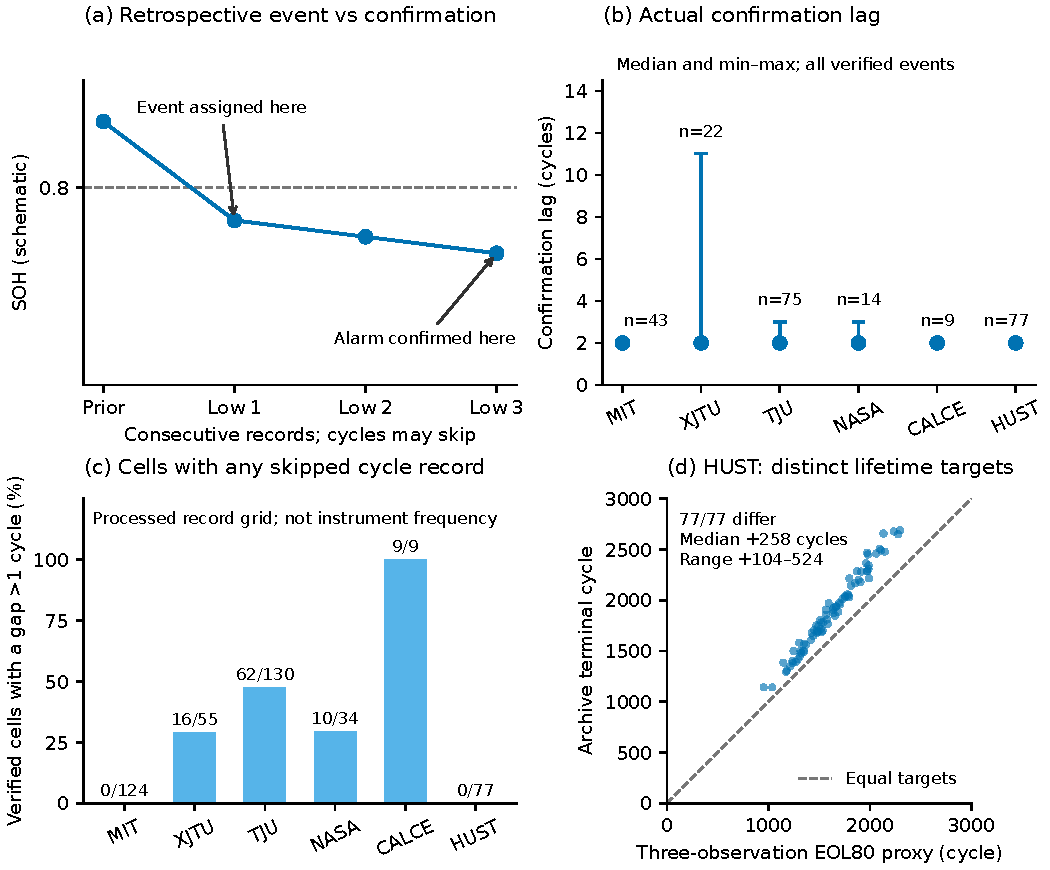
\includegraphics[width=\linewidth]{../figures_v4/fig_v5_endpoint_observation.pdf}
\caption{(a) Schematic only: event assignment precedes confirmation. (b) Actual median and minimum--maximum confirming-cycle lag for all confirmed verified events; n counts events, not cycle-100 eligible cells. (c) Actual cells containing at least one observed cycle gap larger than one; labels give affected/verified cells. (d) Actual paired HUST targets for 77 cells, with equal axes and the equality line. The archive terminal cycle and reconstructed three-observation EOL80 proxy are distinct outcomes.}
\end{figure}

Each source card records provenance/endpoint, landmark cohort/events, scoring range and last risk set, horizon discrepancy, calibration budget and evaluation size, group labels and chronology. \path{source_evidence_cards.csv} stores six aggregate cards. The maximum mean-risk discrepancy is the largest absolute difference between XGB-AFT and held-out KM source-mean event risk over supported horizons.
\begin{center}\small
\begin{minipage}{\linewidth}\centering
\captionof{table}{Reusable source-card index. Values summarize source-specific eligibility, horizon support, risk discrepancy and calibration/evaluation counts.}\label{tab:S6}
\begin{tabular}{lrrrrr}\toprule
Source & N/E & Last cycle & At risk after & Max risk gap & Cal./eval.\\\midrule
MIT & 124/43 & 1000 & 29 & 0.168 & 25/99\\
XJTU & 39/21 & 500 & 16 & 0.041 & 8/31\\
TJU & 119/75 & 1000 & 2 & 0.275 & 24/95\\
NASA & 8/3 & 125 & 3 & 0.337 & 2/6\\
CALCE & 9/9 & 500 & 8 & 0.579 & 2/7\\
HUST & 77/77 & 2000 & 8 & 0.688 & 16/61\\
\bottomrule\end{tabular}\end{minipage}
\end{center}
\textbf{Use in a subsequent energy study.} Specify an action-related capacity endpoint and its measurement cadence; check every requested cycle against supported horizons and risk sets; state whether target labels are used and retain separate evaluation cells; verify label definitions on a new source or certified calendar cohort. A pack or dispatch study must additionally validate the cell-to-pack mapping and compare decisions on common operating data with explicit reliability/cost losses. The card organizes descriptive evidence for those checks. Operational pass/fail thresholds require validation against the proposed actions and losses.

\section*{S8. Training resampling and analysis consistency}
Table~\ref{tab:S7} summarizes the valid training-resampling ranges.
The added sensitivity refits XGB-AFT and pooled KM after 200 within-source cell resamples of the five training sources for each estimable cycle-100 target (1000 draws, 2000 model fits). Training-source sample sizes are preserved. The selected configurations, seed 0, original target cells and original scoring grid remain fixed. Refitting uses training-source cells with the previously selected configurations. NASA has one scoring horizon and is excluded from integrated-score refits. The quantiles describe training-sample sensitivity conditional on those fixed settings and full scoring support.
\begin{center}\small
\begin{minipage}{\linewidth}\centering
\captionof{table}{Training-sample resampling sensitivity conditional on selected configurations and full scoring support. Valid counts identify unavailable draws.}\label{tab:S7}
\begin{tabular}{lrrrr}\toprule
Source & Valid/200 & XGB IBS [2.5\%,97.5\%] & $\Delta$(XGB--KM) range & Lower-IBS draws\\\midrule
MIT & 200 & [0.138, 0.248] & [-0.025, +0.085] & 118\\
XJTU & 200 & [0.052, 0.062] & [-0.006, +0.005] & 130\\
TJU & 200 & [0.148, 0.239] & [-0.194, -0.079] & 200\\
NASA & 0 & -- & -- & --\\
CALCE & 200 & [0.099, 0.369] & [+0.056, +0.327] & 0\\
HUST & 175 & [0.133, 0.182] & [-0.145, -0.063] & 175\\
\bottomrule\end{tabular}\end{minipage}
\end{center}
For HUST, 25/200 draws cannot score pooled KM at the original longest horizon because the resampled training follow-up lacks that support. They remain unavailable; the reported paired ranges use 175 valid draws. The ranges condition on full support in both models; the horizon grid is held fixed. \path{training_resampling_protocol.json}, \path{training_resampling_summary.csv} and the local resample records supply the settings and outputs.

The consistency audit checks recorded within-source protocol input hashes, benchmark/reference labels and AFT locations, current borrowed AFT scales, group counts, the common selection objective and endpoint-script configuration linkage. All executable equality checks pass. Historical endpoint per-fit hashes were not recorded; the current check verifies the script's configuration linkage. XJTU's four eligible batches and TJU's three subsets provide within-archive group controls. The source count remains six.

These additions are post hoc exploratory revision analyses conditional on the selected configurations and six existing archives. Hyperparameter-selection uncertainty and population variation across new sources require further evaluation. Calendar-time validation requires certified experiment start dates, which are unavailable in the current schema. Prospective and physical pack validation require independent cohorts and operating data.
\section*{S9. Independent external validation and decision proxy}
The corrected frozen branch uses the stored historical probabilities and median predictions. Cox/RSF risks were recovered with explicit historical refits reproducing all six originally stored probability points exactly. Event rows use EOL80, not terminal observation; reported IBS is trapezoidal and larger risk denotes earlier endpoint. Only five common scoring points remain: 125/250/500/750/1000. Canonical refits are a separate protocol with own-landmark six-fold source tuning and Python 3.11. Both versions and their 2000 paired-draw contrasts are supplied as aggregate tables.


\begin{table}[H]\centering\scriptsize
\caption{Corrected frozen and canonical external metrics at both landmarks; all rows use 47 complete processed-series cells and the five-point grid.}\label{tab:S8}
\begin{tabular*}{\linewidth}{@{\extracolsep{\fill}}llllll}\toprule
L & Version & Model & IBS & C & MedAPE (\%)\\\midrule
50 & Frozen & KM & 0.116 & 0.500 & 6.9\\
50 & Frozen & LN-AFT & 0.070 & 0.603 & 9.1\\
50 & Frozen & Cox & 0.077 & 0.610 & 12.4\\
50 & Frozen & RSF & 0.089 & 0.509 & 17.6\\
50 & Frozen & XGB-AFT & 0.062 & 0.585 & 22.7\\
100 & Frozen & KM & 0.114 & 0.500 & 6.9\\
100 & Frozen & LN-AFT & 0.075 & 0.610 & 12.8\\
100 & Frozen & Cox & 0.070 & 0.611 & 14.1\\
100 & Frozen & RSF & 0.208 & 0.618 & 55.8\\
100 & Frozen & XGB-AFT & 0.054 & 0.592 & 34.8\\
50 & v6 & KM & 0.116 & 0.500 & 6.9\\
50 & v6 & LN-AFT & 0.070 & 0.603 & 9.1\\
50 & v6 & Cox & 0.077 & 0.610 & 12.4\\
50 & v6 & RSF & 0.089 & 0.509 & 17.6\\
50 & v6 & XGB-AFT & 0.065 & 0.589 & 71.5\\
100 & v6 & KM & 0.114 & 0.500 & 6.9\\
100 & v6 & LN-AFT & 0.070 & 0.617 & 12.0\\
100 & v6 & Cox & 0.070 & 0.611 & 14.1\\
100 & v6 & RSF & 0.160 & 0.602 & 46.6\\
100 & v6 & XGB-AFT & 0.056 & 0.594 & 30.8\\
\bottomrule\end{tabular*}\end{table}

\textbf{Historical derating proxy.} The original replay has XGB mean normalized proxy cost 1.1192 versus fixed 1.0700 (+4.60\%); late actions change from 3/47 to 2/47. All EOL80 endpoints exceed cycle 500, so replacement and derating at 500 have zero pre-action endpoint deficit. Their labels do not identify separate service or degradation effects. The original deficit is a record-sum capacity-deficit proxy, not a cycle-width integral; its cost coefficients cannot be carried into an integrated quantity without unit changes. These adverse historical results are retained but are not the v6 primary decision analysis.


\begin{table}[H]\centering\scriptsize
\caption{Historical action proxy, retained for traceability; no independent derating utility is identified.}\label{tab:S9}
\begin{tabular*}{\linewidth}{@{\extracolsep{\fill}}lll}\toprule
Model & Mean proxy cost & Late count / 47\\\midrule
cox & 1.0700 & 3\\
km & 1.3097 & 0\\
lognormal\_aft & 1.0700 & 3\\
rsf & 1.3097 & 0\\
xgb\_aft & 1.1192 & 2\\
fixed\_baseline & 1.0700 & 3\\
oracle & 1.0000 & 0\\
\bottomrule\end{tabular*}\end{table}


\section*{S10. Paired source-correction intervals}
Table~\ref{tab:S10} gives the source-correction contrasts and valid paired draws.
The cycle-100 contrast is corrected minus historical training IBS on the common verified target cells. Both branches use the original source-selected configuration and seed 0. Predictions are frozen during 2000 paired target-cell bootstrap draws; both branches and both model families share sampled indices within each source. Target censoring KM is re-estimated in each draw, and all original horizons must retain support (censor survival at least 0.10 and horizon below maximum follow-up). Draws lacking full support are unavailable. Intervals are exploratory, unadjusted pointwise percentile 95\% intervals conditional on the held-out source and retained support; they omit retraining and between-source variation. Cells are the resampling units, without modeling within-archive batch dependence. The contrast evaluates joint corrections rather than individual causal parser effects.
\begin{center}\small
\begin{minipage}{\linewidth}\centering
\captionof{table}{Paired source-correction intervals. Delta IBS is corrected minus historical training IBS; intervals are exploratory pointwise percentiles conditional on retained support.}\label{tab:S10}
\begin{tabular}{llrrrr}\toprule
Source & Model & N & $\Delta$IBS & 95\% interval & Valid/2000\\\midrule
MIT & XGB-AFT & 124 & +0.0037 & [+0.0004, +0.0068] & 2000\\
MIT & Cox & 124 & +0.0134 & [+0.0067, +0.0230] & 2000\\
XJTU & XGB-AFT & 39 & -0.0008 & [-0.0030, +0.0014] & 2000\\
XJTU & Cox & 39 & +0.0066 & [+0.0036, +0.0103] & 2000\\
TJU & XGB-AFT & 119 & +0.0000 & [+0.0000, +0.0000] & 1780\\
TJU & Cox & 119 & +0.0000 & [+0.0000, +0.0000] & 1780\\
NASA & XGB-AFT & 8 & -- & -- & --\\
NASA & Cox & 8 & -- & -- & --\\
CALCE & XGB-AFT & 9 & +0.0819 & [+0.0467, +0.1115] & 2000\\
CALCE & Cox & 9 & +0.0077 & [-0.0014, +0.0173] & 2000\\
HUST & XGB-AFT & 77 & -0.0027 & [-0.0056, +0.0003] & 2000\\
HUST & Cox & 77 & +0.0010 & [+0.0006, +0.0013] & 2000\\
\bottomrule\end{tabular}\end{minipage}
\end{center}
TJU's branches have identical risk predictions; its [0,0] interval is a conditional identity contrast. NASA has only one supported horizon and no IBS. All 2000 draws retain full support except TJU (1780). The inset in main Figure 5 repeats MIT, XJTU and HUST estimates with enlarged x limits [-0.006,0.025]. Settings, package versions, input hashes and valid counts are in \path{source_correction_bootstrap_protocol.json} and \path{source_correction_bootstrap_summary.csv}.

\section*{v6.2 production correction and frozen-grid evidence}
The v6.2 production path applies the frozen nearest-feasible opportunity rule to B0 separately for every $(L,H,\delta)$ setting. The complete 504-scenario audit changes 196 planned actions, 28 effective actions, 168 maintenance flags and 20 evaluable losses; the 20 losses comprise 12 decreases and 8 increases. All finite loss values match the round-4 corrected audit on their 408-scenario common support; the remaining 96 values remain unavailable under the event-support contract. Early and late cycle fields are retained in the v6.2 output, while round 4 did not publish corresponding comparable fields. No probability clipping is used for invalid Cox fits.

The CALCE far-tail diagnostic is reproduced from the frozen event-error table. At landmark 100, the native one-observation cohort has seven events and LN-AFT MedAPE 31905.8\%, MAE 111075.3 cycles and MedAE 40520.4 cycles; its median predicted residual life is 40547.4 cycles. The seven-event common three-observation cohort has MedAPE 3508.4\%, MAE 37742.9 cycles and MedAE 20313.8 cycles, with median predicted residual life 20792.8 cycles. These are observed-endpoint proxy results and do not establish physical failure timing.

Figure~\ref{fig:v62mitgrid} reports the frozen MIT observation-grid replay: 43/124 confirmed events at one-cycle spacing, 34/124 at five-cycle spacing and 0/124 at twenty-cycle spacing; right-censoring fractions are 0.653, 0.726 and 1.000. The grid changes the observed-record confirmation contract and support; it does not show that physical failures disappeared. Figure~\ref{fig:v62b0} records the complete B0 correction counts. The matched-support selection tables retain fixed-prediction S-I/S-M/S-D results, loss-only S-D as a sensitivity analysis, and complete-refit results as a separate estimand. Model-winner stability, prediction-error stability and action stability are therefore reported separately.

\begin{figure}[htbp]\centering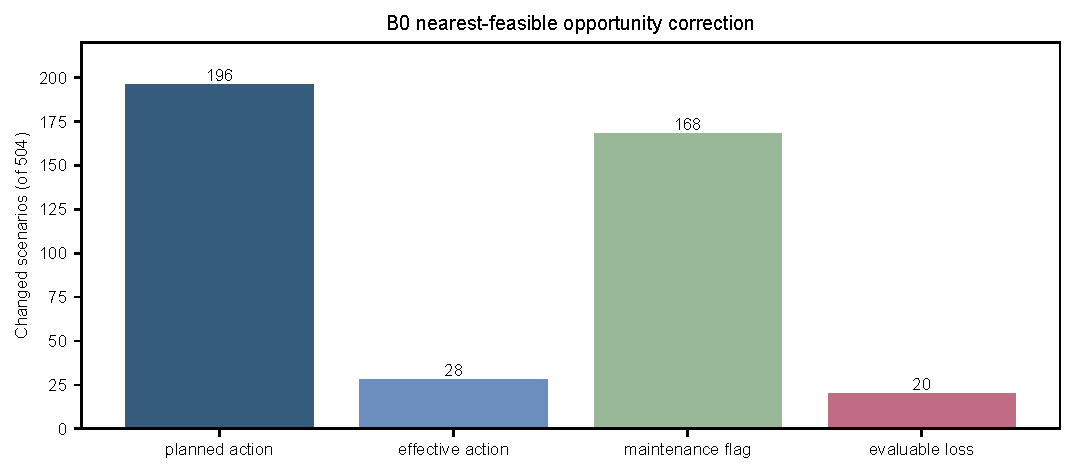
\includegraphics[width=0.94\linewidth]{../figures_v6_2/fig_v6_2_b0_repair.pdf}\caption{B0 production correction across all 504 settings. Counts are computed from the v6.2 old/new field audit; unsupported losses are not imputed.}\label{fig:v62b0}\end{figure}
\begin{figure}[htbp]\centering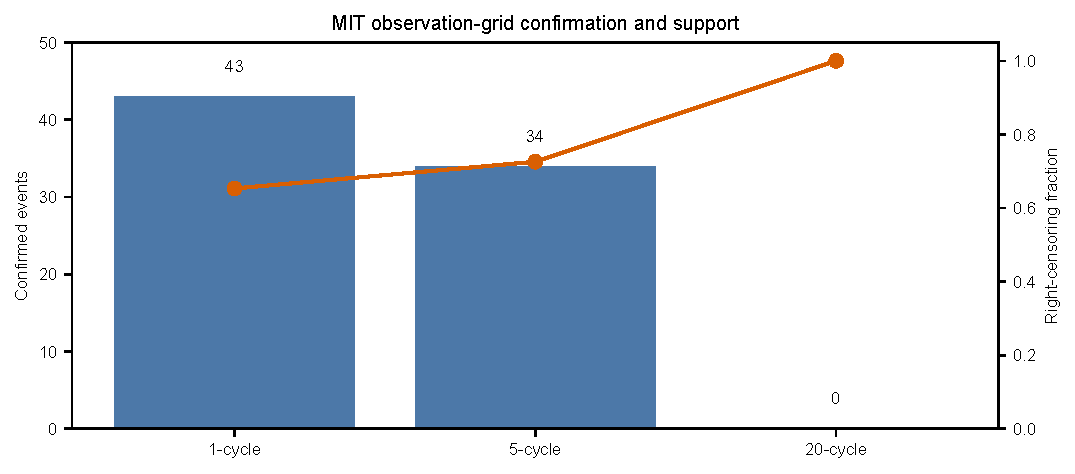
\includegraphics[width=0.94\linewidth]{../figures_v6_2/fig_v6_2_mit_grid.pdf}\caption{MIT observation-grid confirmation and support from the frozen round-6 grid table.}\label{fig:v62mitgrid}\end{figure}

\section*{Release-path audit (v6.2)}
The production model bank now imports the versioned candidate library \path{production_model_library.py}. Cox survival is evaluated in log-domain form, $\exp[-H_0(t)\exp\{\eta\}]$, with invalid cumulative hazards, non-finite predictors, non-monotone curves and unconverged fits retained as unavailable. No probability clipping is applied. The release code version is \texttt{v6.2-b0-nearest-feasible-20261010}; the full input, environment and code hashes are in \path{release_reproducibility_receipt.json}.

The clean-runtime replay performed ten fresh external fits under the locked Python 3.11 environment. Risk scores and supported survival curves matched the cached release within $10^{-7}$. Configuration candidates and winners were unchanged. Nine Cox IBS cells differed only in the last floating-point digits (maximum absolute difference below $2\times10^{-16}$); all other benchmark metrics, event-median coverage, selection labels, action schedules and timing-loss fields were unchanged. Historical caches and outputs remain preserved in their original directories.

The primary three-selector analysis uses the same common estimable validation-source intersection for S-I, S-M and S-D. The loss-only S-D support is retained as a separately labelled sensitivity because its estimability gate can differ. All NA fields retain their reason: unsupported horizons, censoring survival below the floor, no complete event-median support or no observed event. The controlled MIT grid replay reports 43/124, 34/124 and 0/124 confirmed events at 1-, 5- and 20-cycle post-landmark observation intervals, with right-censoring fractions 0.653, 0.726 and 1.000. Fixed-prediction and complete-refit outputs are separate. The grid replay changes an observed-record endpoint contract; it does not identify a physical failure time.

\section*{S11. Replacement contracts, selection and complete sensitivity}
The main replacement analysis has 2 landmarks, 7 targets, 3 windows, 4 penalty ratios and 3 opportunity intervals (504 combinations). \path{replacement_metrics.csv} records loss, weighted early/late cycles, late known counts, known outcomes, maintenance counts, fallback counts, planned/effective means and support reasons. \path{replacement_pairwise_bootstrap.csv} records 2000 paired-draw contrasts and valid counts. \path{selection_results.csv} records each family's criterion and common estimable validation sources. \path{selection_disagreements.csv} records family/action disagreements. No adverse or NA scenario is omitted. Full source label access and hashed training membership are recorded in \path{replacement_protocol.json}.

The estimand is the restricted dimensionless timing loss in the main equations. B0 selects the feasible opportunity nearest to 1000 for each $(L,H,\delta)$, with earlier ties; B1 is source-validation selected; B2 equals KM-Pd. Pm uses nearest candidate median timing and explicit B1 fallback; Pd uses exact predictive integrals. An action at H and continued operation beyond H have identical restricted loss but different action flags. Oracle zero loss is a retrospective lower bound only. Scenario ratios are not measured economic prices. Loss uncertainty fixes all selected families and fits; training variation is not included. The old 200 training-resample results in S8 remain a separate internal fixed-configuration sensitivity.

Marginal censor KM weights require within-source independent censoring. Events by H use G(Y-), follow-up covering H uses G(H), and early censored outcomes are unknown; no terminal endpoint is imputed. The floor is 0.10. Complete external events yield direct means. H1500 decision loss is estimable for complete ISEA events under source prediction support although conservative Brier scoring at 1500 is unavailable. All scenarios are post hoc because ISEA had been examined before their design. Target exclusion from fitting and selection does not make the scenario design independent. The paired intervals fix that design and do not account for its selection. A new confirmatory source must be inspected only after freezing the endpoint, windows, penalty ratios and opportunities. For the 44/47 complete ISEA events beyond H1000, truncation gives U=H and B0 effective action a=H, hence zero restricted loss. This does not convert their observed events into censored outcomes; it explains the window dependence of the comparison.


\begin{table}[H]\centering\scriptsize
\caption{Reference replacement-selection consequences at L100/H1000/rho4/50-cycle opportunities. Entries are source-specific original point estimates; NASA loss is NA.}\label{tab:S11}
\begin{tabular*}{\linewidth}{@{\extracolsep{\fill}}lllllll}\toprule
Source & M model & I model & D model & M loss & I loss & D loss\\\midrule
MIT & RSF & XGB-AFT & XGB-AFT & 0.203 & 0.584 & 0.584\\
XJTU & RSF & Cox & KM & 0.227 & 0.267 & 0.202\\
TJU & XGB-AFT & KM & KM & 0.415 & 0.499 & 0.499\\
NASA & RSF & RSF & RSF & NA & NA & NA\\
CALCE & RSF & XGB-AFT & RSF & 0.406 & 0.493 & 0.406\\
HUST & KM & Cox & KM & 0.610 & 0.500 & 0.610\\
ISEA & Cox & RSF & RSF & 0.489 & 0.696 & 0.696\\
\bottomrule\end{tabular*}\end{table}

\textbf{Endpoint sensitivity.} \path{endpoint_replacement_metrics.csv} uses 119 common TJU cells and a grid intersected across four rules and five models. Primary source-only configurations are frozen rather than retuned for each endpoint. \path{endpoint_selection_results.csv} records source-only choices. This conditional sensitivity concerns four distinct outcomes. The original observation audit separates event and confirmation cycles.

\textbf{HUST target sensitivity.} \path{hust_training_target_sensitivity.csv} changes only HUST training labels from EOL80 to its audited archive RUL terminal target, holding features, cells, primary configurations and held-out EOL80 scoring fixed. This is not an optimized archive-RUL benchmark. The HUST-held-out branches are identical; the archive target is not declared erroneous.

\textbf{Input and runtime.} \path{external_input_audit.json} records 10,686 TDS rows, 3,510,013 exact overlaps, five-cycle spacing and unavailable 47-to-48 raw-cell mapping. Upstream online availability remains unverified. \path{requirements-lock.txt} pins the full canonical dependency inventory; \path{clean_runtime_verification.json} records installation into an independent environment and ten fresh full-source external fits reproducing canonical predictions within 1e-7. Frozen historical recovery separately uses Python 3.12. \path{analysis_verification.json} records event, probability, loss, baseline and paired-contrast gates. No mixture of temporary dependency directories is used by canonical analysis.

\textbf{Features.} First valid capacity (Ah), last SOH, OLS slope times 1000 (SOH per 1000 cycles), drops from first normalized SOH at cycles 10 and floor(L/2), population SOH standard deviation, count of consecutive record rises exceeding 0.001 and signed largest rise form the eight inputs. All feature records are at/before L; missing early drops use training-only median imputation. Exact formulas and source locators are in \path{feature_definitions.md}. Raw, cell/cycle tables and fit caches remain outside the review bundle.


\section*{S12. Event-cycle median availability and NASA single-point scoring}
MedAPE uses absolute event cycles, $100\operatorname{median}\left(\frac{|\widehat T-T|}{T}\right)$, on observed events with finite predicted medians. Table~\ref{tab:median_availability} gives the numerator and the full event denominator; no unavailable median is replaced by a maintenance fallback. Reporting on a finite subset differs from the selection gate: S-M, S-I and S-D all require every event median and an estimable IBS for all five families on each common validation source. HUST Cox coverage is 36/77 at L50 and 31/77 at L100. Its subset error does not summarize all HUST events. NASA has only the cycle-125 Brier point in Table~\ref{tab:nasa125}; IBS remains unavailable because a single point cannot define the normalized integral.
{\scriptsize
\begin{longtable}{@{\extracolsep{\fill}}lllllll}
\caption{Finite predicted event medians / all observed events. The error population is the finite subset.}\label{tab:median_availability}\\
\toprule
L & Source & KM & LN-AFT & Cox & RSF & XGB-AFT\\\midrule
\endfirsthead
\toprule
L & Source & KM & LN-AFT & Cox & RSF & XGB-AFT\\\midrule
\endhead
\bottomrule\endfoot
50 & MIT & 43/43 & 43/43 & 43/43 & 43/43 & 43/43\\
50 & XJTU & 21/21 & 21/21 & 21/21 & 21/21 & 21/21\\
50 & TJU & 75/75 & 75/75 & 75/75 & 75/75 & 75/75\\
50 & NASA & 5/5 & 5/5 & 5/5 & 5/5 & 5/5\\
50 & CALCE & 9/9 & 9/9 & 9/9 & 9/9 & 9/9\\
50 & HUST & 77/77 & 77/77 & 36/77 & 77/77 & 77/77\\
50 & ISEA & 47/47 & 47/47 & 47/47 & 47/47 & 47/47\\
100 & MIT & 43/43 & 43/43 & 43/43 & 43/43 & 43/43\\
100 & XJTU & 21/21 & 21/21 & 21/21 & 21/21 & 21/21\\
100 & TJU & 75/75 & 75/75 & 75/75 & 75/75 & 75/75\\
100 & NASA & 3/3 & 3/3 & 3/3 & 3/3 & 3/3\\
100 & CALCE & 9/9 & 9/9 & 9/9 & 9/9 & 9/9\\
100 & HUST & 77/77 & 77/77 & 31/77 & 77/77 & 77/77\\
100 & ISEA & 47/47 & 47/47 & 47/47 & 47/47 & 47/47\\
\end{longtable}}
{\scriptsize
\begin{longtable}{@{\extracolsep{\fill}}lllllll}
\caption{NASA Brier at absolute cycle 125. N is the landmark cohort; events and risk set refer to cycle 125. All listed points pass the scoring support gate; IBS is NA.}\label{tab:nasa125}\\
\toprule
L & Model & N & Events & At risk & $G(125)$ & Brier\\\midrule
\endfirsthead
\toprule
L & Model & N & Events & At risk & $G(125)$ & Brier\\\midrule
\endhead
\bottomrule\endfoot
50 & KM & 11 & 4 & 3 & 0.568 & 0.520000\\
50 & LN-AFT & 11 & 4 & 3 & 0.568 & 0.994001\\
50 & Cox & 11 & 4 & 3 & 0.568 & 0.520000\\
50 & RSF & 11 & 4 & 3 & 0.568 & 0.520000\\
50 & XGB-AFT & 11 & 4 & 3 & 0.568 & 0.421518\\
100 & KM & 8 & 2 & 3 & 0.625 & 0.400000\\
100 & LN-AFT & 8 & 2 & 3 & 0.625 & 0.909318\\
100 & Cox & 8 & 2 & 3 & 0.625 & 0.400000\\
100 & RSF & 8 & 2 & 3 & 0.625 & 0.400000\\
100 & XGB-AFT & 8 & 2 & 3 & 0.625 & 0.362080\\
\end{longtable}}

\section*{S13. Common validation sources, exclusion diagnostics and selection margins}
The inner-validation audit reads predictions from the original input-fingerprinted caches and reproduces all 1512 selected families, criterion values and B1 actions without fitting. A source enters B1 only when all five predictions are fitted, their training follow-up covers H, and restricted-loss censoring weights are available. A common family-selection source additionally needs estimable IBS and complete event-median availability in all five families. Each criterion averages equally over that same intersection. Table~\ref{tab:selection_support} shows the reference sets; these are validation sets, not the complete outer training set.
{\scriptsize
\begin{longtable}{@{\extracolsep{\fill}}lllll}
\caption{Reference validation membership at L100/H1000/rho4/delta50. Source lists use the abbreviations in S1.}\label{tab:selection_support}\\
\toprule
Target & Common family sources & N & B1 sources & N\\\midrule
\endfirsthead
\toprule
Target & Common family sources & N & B1 sources & N\\\midrule
\endhead
\bottomrule\endfoot
MIT & XJTU, TJU, CALCE, HUST & 4 & XJTU, TJU, CALCE, HUST & 4\\
XJTU & MIT, TJU, CALCE & 3 & MIT, TJU, CALCE, HUST & 4\\
TJU & MIT, XJTU, CALCE & 3 & MIT, XJTU, CALCE, HUST & 4\\
NASA & MIT, XJTU, TJU, CALCE & 4 & MIT, XJTU, TJU, CALCE, HUST & 5\\
CALCE & MIT, XJTU, TJU & 3 & MIT, XJTU, TJU, HUST & 4\\
HUST & MIT, CALCE & 2 & MIT, XJTU, TJU, CALCE & 4\\
ISEA & MIT, XJTU, TJU, CALCE & 4 & MIT, XJTU, TJU, CALCE, HUST & 5\\
\end{longtable}}
{\scriptsize
\begin{longtable}{@{\extracolsep{\fill}}llllll}
\caption{ISEA validation membership by landmark and window. Membership was checked to be identical across all 12 rho/delta combinations within each row.}\label{tab:window_support}\\
\toprule
L & H & Common family sources & N & B1 sources & N\\\midrule
\endfirsthead
\toprule
L & H & Common family sources & N & B1 sources & N\\\midrule
\endhead
\bottomrule\endfoot
50 & 500 & MIT, XJTU, TJU, CALCE & 4 & MIT, XJTU, TJU, CALCE, HUST & 5\\
50 & 1000 & MIT, XJTU, TJU, CALCE & 4 & MIT, XJTU, TJU, CALCE, HUST & 5\\
50 & 1500 & XJTU, TJU, CALCE & 3 & XJTU, TJU, CALCE, HUST & 4\\
100 & 500 & MIT, XJTU, TJU, CALCE & 4 & MIT, XJTU, TJU, CALCE, HUST & 5\\
100 & 1000 & MIT, XJTU, TJU, CALCE & 4 & MIT, XJTU, TJU, CALCE, HUST & 5\\
100 & 1500 & XJTU, TJU, CALCE & 3 & XJTU, TJU, CALCE, HUST & 4\\
\end{longtable}}
{\scriptsize
\begin{longtable}{@{\extracolsep{\fill}}llllll}
\caption{ISEA reference point-selection margins. Gaps are runner-up minus winner in the criterion's own units; they are not selection-stability intervals.}\label{tab:selection_margins}\\
\toprule
Rule & Winner & Value & Runner-up & Value & Gap\\\midrule
\endfirsthead
\toprule
Rule & Winner & Value & Runner-up & Value & Gap\\\midrule
\endhead
\bottomrule\endfoot
S-M & Cox & 76.231575 & RSF & 76.612027 & 0.380452\\
S-I & RSF & 0.133956 & Cox & 0.136376 & 0.002420\\
S-D & RSF & 0.289603 & KM & 0.318454 & 0.028851\\
\end{longtable}}
{\scriptsize
\begin{longtable}{@{\extracolsep{\fill}}llllll}
\caption{ISEA source-level exclusion summary. Time/fit means the shared prediction-support gate fails; Censor means restricted-loss censor support fails. IBS/median identifies families failing either additional gate.}\label{tab:selection_exclusions}\\
\toprule
L & H & Validation source & B1 & Common & First gate / family\\\midrule
\endfirsthead
\toprule
L & H & Validation source & B1 & Common & First gate / family\\\midrule
\endhead
\bottomrule\endfoot
50 & 500 & MIT & yes & yes & Included\\
50 & 500 & XJTU & yes & yes & Included\\
50 & 500 & TJU & yes & yes & Included\\
50 & 500 & NASA & no & no & Censor\\
50 & 500 & CALCE & yes & yes & Included\\
50 & 500 & HUST & yes & no & IBS/median: Cox\\
50 & 1000 & MIT & yes & yes & Included\\
50 & 1000 & XJTU & yes & yes & Included\\
50 & 1000 & TJU & yes & yes & Included\\
50 & 1000 & NASA & no & no & Censor\\
50 & 1000 & CALCE & yes & yes & Included\\
50 & 1000 & HUST & yes & no & IBS/median: Cox\\
50 & 1500 & MIT & no & no & Censor\\
50 & 1500 & XJTU & yes & yes & Included\\
50 & 1500 & TJU & yes & yes & Included\\
50 & 1500 & NASA & no & no & Censor\\
50 & 1500 & CALCE & yes & yes & Included\\
50 & 1500 & HUST & yes & no & IBS/median: Cox\\
100 & 500 & MIT & yes & yes & Included\\
100 & 500 & XJTU & yes & yes & Included\\
100 & 500 & TJU & yes & yes & Included\\
100 & 500 & NASA & no & no & Censor\\
100 & 500 & CALCE & yes & yes & Included\\
100 & 500 & HUST & yes & no & IBS/median: Cox\\
100 & 1000 & MIT & yes & yes & Included\\
100 & 1000 & XJTU & yes & yes & Included\\
100 & 1000 & TJU & yes & yes & Included\\
100 & 1000 & NASA & no & no & Censor\\
100 & 1000 & CALCE & yes & yes & Included\\
100 & 1000 & HUST & yes & no & IBS/median: Cox\\
100 & 1500 & MIT & no & no & Censor\\
100 & 1500 & XJTU & yes & yes & Included\\
100 & 1500 & TJU & yes & yes & Included\\
100 & 1500 & NASA & no & no & Censor\\
100 & 1500 & CALCE & yes & yes & Included\\
100 & 1500 & HUST & yes & no & IBS/median: Cox\\
\end{longtable}}
\path{reporting_selection_diagnostics.csv} contains all 1080 L/outer-target/H/validation-source/model records, fitted flags, training follow-up, IBS, finite/all-event counts, censor reasons and every failed condition, in addition to the first exclusion gate. \path{reporting_selection_support.csv} and \path{reporting_criterion_margins.csv} retain all 504 scenario sets and 1512 criterion margins. Overlapping validation-source sets, source-specific scoring grids and two-source intersections constrain interpretation; none is an independent replicate of transfer to a new source.

\section*{S14. Complete scenario contrasts and timing decomposition}
Figure~\ref{fig:scenarios} displays every ISEA scenario for both contrasts (144 entries). Positive D-minus-M/I means greater decision-selection loss; zero and NA have distinct markings. Windows contain 0, 3 and 47 observed external events, respectively. Table~\ref{tab:scenario_summary} summarizes all 1008 contrasts across seven targets: each row counts its 12 rho/delta combinations. The 84 rows are a sensitivity inventory, not independent hypothesis tests. Conditional intervals, selected families, support reasons and valid paired-draw counts are retained in \path{reporting_scenario_contrasts.csv}.
\begin{figure}[htbp]\centering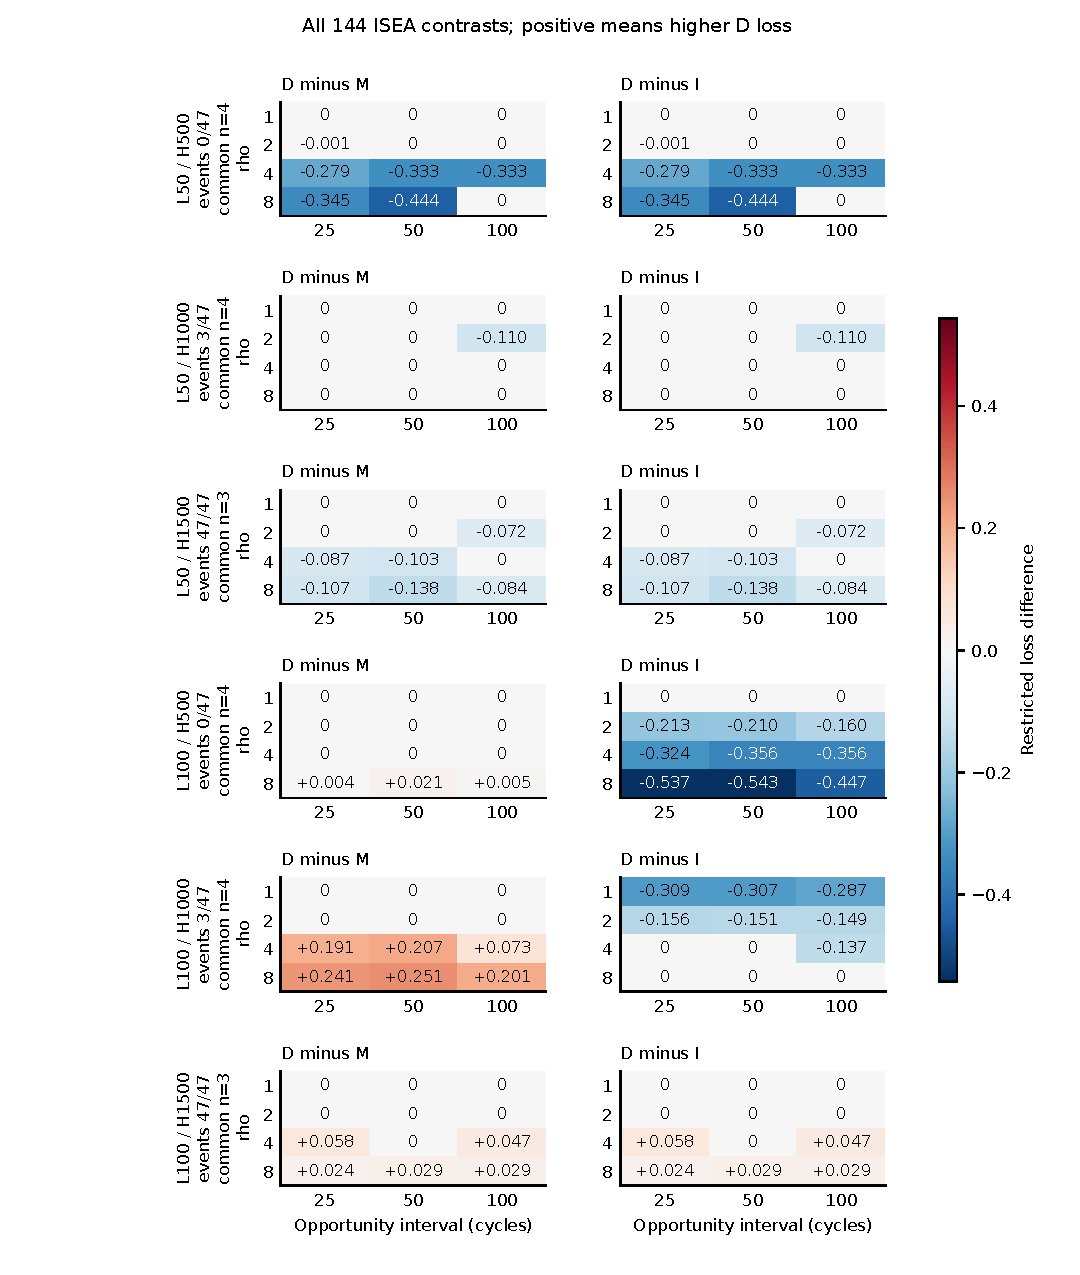
\includegraphics[width=0.98\linewidth]{../figures_v6/fig_v6_scenario_contrasts.pdf}
\caption{Complete ISEA restricted-loss differences. Rows group landmark and H; each small grid has rho=1,2,4,8 downwards and delta=25,50,100 across. Common validation-source count and event count appear in each row label. All panels use one symmetric color scale; numbers are original point estimates. Exact zero is printed as 0; NA indicates unavailable support. Contrasts condition on the same processed external source; no selection of a favorable window or scenario is implied.}\label{fig:scenarios}\end{figure}
{\scriptsize
\begin{longtable}{@{\extracolsep{\fill}}llllllll}
\caption{All target/landmark/window sign counts. Each contrast row contains 12 scenarios; NA is retained separately. D-M and D-I denote decision minus median and decision minus IBS selection.}\label{tab:scenario_summary}\\
\toprule
L & Target & H & Contrast & Negative & Zero & Positive & NA\\\midrule
\endfirsthead
\toprule
L & Target & H & Contrast & Negative & Zero & Positive & NA\\\midrule
\endhead
\bottomrule\endfoot
50 & MIT & 500 & D-M & 0 & 0 & 12 & 0\\
50 & MIT & 500 & D-I & 4 & 8 & 0 & 0\\
50 & MIT & 1000 & D-M & 3 & 0 & 9 & 0\\
50 & MIT & 1000 & D-I & 9 & 0 & 3 & 0\\
50 & MIT & 1500 & D-M & 0 & 0 & 0 & 12\\
50 & MIT & 1500 & D-I & 0 & 0 & 0 & 12\\
50 & XJTU & 500 & D-M & 1 & 5 & 6 & 0\\
50 & XJTU & 500 & D-I & 0 & 9 & 3 & 0\\
50 & XJTU & 1000 & D-M & 1 & 5 & 6 & 0\\
50 & XJTU & 1000 & D-I & 4 & 4 & 4 & 0\\
50 & XJTU & 1500 & D-M & 2 & 6 & 4 & 0\\
50 & XJTU & 1500 & D-I & 3 & 6 & 3 & 0\\
50 & TJU & 500 & D-M & 3 & 3 & 6 & 0\\
50 & TJU & 500 & D-I & 0 & 12 & 0 & 0\\
50 & TJU & 1000 & D-M & 0 & 4 & 8 & 0\\
50 & TJU & 1000 & D-I & 7 & 5 & 0 & 0\\
50 & TJU & 1500 & D-M & 3 & 3 & 6 & 0\\
50 & TJU & 1500 & D-I & 6 & 6 & 0 & 0\\
50 & NASA & 500 & D-M & 0 & 0 & 0 & 12\\
50 & NASA & 500 & D-I & 0 & 0 & 0 & 12\\
50 & NASA & 1000 & D-M & 0 & 0 & 0 & 12\\
50 & NASA & 1000 & D-I & 0 & 0 & 0 & 12\\
50 & NASA & 1500 & D-M & 0 & 0 & 0 & 12\\
50 & NASA & 1500 & D-I & 0 & 0 & 0 & 12\\
50 & CALCE & 500 & D-M & 12 & 0 & 0 & 0\\
50 & CALCE & 500 & D-I & 0 & 12 & 0 & 0\\
50 & CALCE & 1000 & D-M & 12 & 0 & 0 & 0\\
50 & CALCE & 1000 & D-I & 3 & 9 & 0 & 0\\
50 & CALCE & 1500 & D-M & 9 & 3 & 0 & 0\\
50 & CALCE & 1500 & D-I & 3 & 9 & 0 & 0\\
50 & HUST & 500 & D-M & 0 & 12 & 0 & 0\\
50 & HUST & 500 & D-I & 0 & 12 & 0 & 0\\
50 & HUST & 1000 & D-M & 0 & 12 & 0 & 0\\
50 & HUST & 1000 & D-I & 0 & 12 & 0 & 0\\
50 & HUST & 1500 & D-M & 0 & 12 & 0 & 0\\
50 & HUST & 1500 & D-I & 0 & 12 & 0 & 0\\
50 & ISEA & 500 & D-M & 6 & 6 & 0 & 0\\
50 & ISEA & 500 & D-I & 6 & 6 & 0 & 0\\
50 & ISEA & 1000 & D-M & 1 & 11 & 0 & 0\\
50 & ISEA & 1000 & D-I & 1 & 11 & 0 & 0\\
50 & ISEA & 1500 & D-M & 6 & 6 & 0 & 0\\
50 & ISEA & 1500 & D-I & 6 & 6 & 0 & 0\\
100 & MIT & 500 & D-M & 0 & 0 & 12 & 0\\
100 & MIT & 500 & D-I & 6 & 0 & 6 & 0\\
100 & MIT & 1000 & D-M & 5 & 0 & 7 & 0\\
100 & MIT & 1000 & D-I & 1 & 8 & 3 & 0\\
100 & MIT & 1500 & D-M & 0 & 0 & 0 & 12\\
100 & MIT & 1500 & D-I & 0 & 0 & 0 & 12\\
100 & XJTU & 500 & D-M & 0 & 0 & 12 & 0\\
100 & XJTU & 500 & D-I & 0 & 0 & 12 & 0\\
100 & XJTU & 1000 & D-M & 12 & 0 & 0 & 0\\
100 & XJTU & 1000 & D-I & 6 & 6 & 0 & 0\\
100 & XJTU & 1500 & D-M & 4 & 5 & 3 & 0\\
100 & XJTU & 1500 & D-I & 4 & 5 & 3 & 0\\
100 & TJU & 500 & D-M & 6 & 0 & 6 & 0\\
100 & TJU & 500 & D-I & 0 & 12 & 0 & 0\\
100 & TJU & 1000 & D-M & 7 & 0 & 5 & 0\\
100 & TJU & 1000 & D-I & 9 & 3 & 0 & 0\\
100 & TJU & 1500 & D-M & 0 & 6 & 6 & 0\\
100 & TJU & 1500 & D-I & 6 & 6 & 0 & 0\\
100 & NASA & 500 & D-M & 0 & 0 & 0 & 12\\
100 & NASA & 500 & D-I & 0 & 0 & 0 & 12\\
100 & NASA & 1000 & D-M & 0 & 0 & 0 & 12\\
100 & NASA & 1000 & D-I & 0 & 0 & 0 & 12\\
100 & NASA & 1500 & D-M & 0 & 0 & 0 & 12\\
100 & NASA & 1500 & D-I & 0 & 0 & 0 & 12\\
100 & CALCE & 500 & D-M & 6 & 6 & 0 & 0\\
100 & CALCE & 500 & D-I & 12 & 0 & 0 & 0\\
100 & CALCE & 1000 & D-M & 6 & 6 & 0 & 0\\
100 & CALCE & 1000 & D-I & 12 & 0 & 0 & 0\\
100 & CALCE & 1500 & D-M & 0 & 6 & 6 & 0\\
100 & CALCE & 1500 & D-I & 12 & 0 & 0 & 0\\
100 & HUST & 500 & D-M & 4 & 8 & 0 & 0\\
100 & HUST & 500 & D-I & 0 & 11 & 1 & 0\\
100 & HUST & 1000 & D-M & 4 & 8 & 0 & 0\\
100 & HUST & 1000 & D-I & 1 & 3 & 8 & 0\\
100 & HUST & 1500 & D-M & 0 & 12 & 0 & 0\\
100 & HUST & 1500 & D-I & 0 & 0 & 12 & 0\\
100 & ISEA & 500 & D-M & 0 & 9 & 3 & 0\\
100 & ISEA & 500 & D-I & 9 & 3 & 0 & 0\\
100 & ISEA & 1000 & D-M & 0 & 6 & 6 & 0\\
100 & ISEA & 1000 & D-I & 7 & 5 & 0 & 0\\
100 & ISEA & 1500 & D-M & 0 & 7 & 5 & 0\\
100 & ISEA & 1500 & D-I & 0 & 7 & 5 & 0\\
\end{longtable}}
{\scriptsize
\begin{longtable}{@{\extracolsep{\fill}}lllll}
\caption{Exact loss and late-count values supporting main Figure 9. The figure uses discrete rho categories, with loss panels and separate late-count grids; coincident losses are retained without jitter.}\label{tab:discrete_rho}\\
\toprule
H & Policy & $\rho$ & Late / 47 & Loss\\\midrule
\endfirsthead
\toprule
H & Policy & $\rho$ & Late / 47 & Loss\\\midrule
\endhead
\bottomrule\endfoot
500 & B0 & 1 & 0 & 0.000000\\
500 & B1 & 1 & 0 & 0.000000\\
500 & Pd-rsf & 1 & 0 & 0.000000\\
500 & Pd-xgb-aft & 1 & 0 & 0.000000\\
500 & B2 & 1 & 0 & 0.000000\\
500 & B0 & 2 & 0 & 0.000000\\
500 & B1 & 2 & 0 & 0.000000\\
500 & Pd-rsf & 2 & 0 & 0.210106\\
500 & Pd-xgb-aft & 2 & 0 & 0.010638\\
500 & B2 & 2 & 0 & 0.000000\\
500 & B0 & 4 & 0 & 0.000000\\
500 & B1 & 4 & 0 & 0.000000\\
500 & Pd-rsf & 4 & 0 & 0.356383\\
500 & Pd-xgb-aft & 4 & 0 & 0.037234\\
500 & B2 & 4 & 0 & 0.000000\\
500 & B0 & 8 & 0 & 0.000000\\
500 & B1 & 8 & 0 & 0.250000\\
500 & Pd-rsf & 8 & 0 & 0.563830\\
500 & Pd-xgb-aft & 8 & 0 & 0.239362\\
500 & B2 & 8 & 0 & 0.250000\\
1000 & B0 & 1 & 3 & 0.004255\\
1000 & B1 & 1 & 0 & 0.440189\\
1000 & Pd-rsf & 1 & 0 & 0.311348\\
1000 & Pd-xgb-aft & 1 & 3 & 0.027896\\
1000 & B2 & 1 & 3 & 0.004255\\
1000 & B0 & 2 & 3 & 0.008511\\
1000 & B1 & 2 & 0 & 0.495745\\
1000 & Pd-rsf & 2 & 0 & 0.512293\\
1000 & Pd-xgb-aft & 2 & 0 & 0.171868\\
1000 & B2 & 2 & 0 & 0.495745\\
1000 & B0 & 4 & 3 & 0.017021\\
1000 & B1 & 4 & 0 & 0.551300\\
1000 & Pd-rsf & 4 & 0 & 0.695508\\
1000 & Pd-xgb-aft & 4 & 0 & 0.373995\\
1000 & B2 & 4 & 0 & 0.551300\\
1000 & B0 & 8 & 3 & 0.034043\\
1000 & B1 & 8 & 0 & 0.662411\\
1000 & Pd-rsf & 8 & 0 & 0.801891\\
1000 & Pd-xgb-aft & 8 & 0 & 0.596217\\
1000 & B2 & 8 & 0 & 0.662411\\
1500 & B0 & 1 & 3 & 0.090805\\
1500 & B1 & 1 & 0 & 0.371049\\
1500 & Pd-rsf & 1 & 7 & 0.270593\\
1500 & Pd-xgb-aft & 1 & 41 & 0.187158\\
1500 & B2 & 1 & 12 & 0.063450\\
1500 & B0 & 2 & 3 & 0.093541\\
1500 & B1 & 2 & 0 & 0.406763\\
1500 & Pd-rsf & 2 & 3 & 0.406839\\
1500 & Pd-xgb-aft & 2 & 14 & 0.303040\\
1500 & B2 & 2 & 0 & 0.406763\\
1500 & B0 & 4 & 3 & 0.099012\\
1500 & B1 & 4 & 0 & 0.442477\\
1500 & Pd-rsf & 4 & 0 & 0.535182\\
1500 & Pd-xgb-aft & 4 & 1 & 0.327356\\
1500 & B2 & 4 & 0 & 0.442477\\
1500 & B0 & 8 & 3 & 0.109954\\
1500 & B1 & 8 & 0 & 0.513906\\
1500 & Pd-rsf & 8 & 0 & 0.603571\\
1500 & Pd-xgb-aft & 8 & 0 & 0.471353\\
1500 & B2 & 8 & 0 & 0.513906\\
\end{longtable}}
{\scriptsize
\begin{longtable}{@{\extracolsep{\fill}}lllllll}
\caption{ISEA reference rho4/delta50 timing decomposition. Early/late cycles are mean weighted cycle penalties before multiplication by rho; A is mean effective action.}\label{tab:actions_decomposition}\\
\toprule
H & Policy & Early & Late & Late / 47 & Mean A & Loss\\\midrule
\endfirsthead
\toprule
H & Policy & Early & Late & Late / 47 & Mean A & Loss\\\midrule
\endhead
\bottomrule\endfoot
500 & B0 & 0.0 & 0.0 & 0 & 500.0 & 0.000000\\
500 & B1 & 0.0 & 0.0 & 0 & 500.0 & 0.000000\\
500 & B2 & 0.0 & 0.0 & 0 & 500.0 & 0.000000\\
500 & S-M & 0.0 & 0.0 & 0 & 500.0 & 0.000000\\
500 & S-I & 142.6 & 0.0 & 0 & 357.4 & 0.356383\\
500 & S-D & 0.0 & 0.0 & 0 & 500.0 & 0.000000\\
1000 & B0 & 0.0 & 3.8 & 3 & 1000.0 & 0.017021\\
1000 & B1 & 496.2 & 0.0 & 0 & 500.0 & 0.551300\\
1000 & B2 & 496.2 & 0.0 & 0 & 500.0 & 0.551300\\
1000 & S-M & 439.8 & 0.0 & 0 & 556.4 & 0.488652\\
1000 & S-I & 626.0 & 0.0 & 0 & 370.2 & 0.695508\\
1000 & S-D & 626.0 & 0.0 & 0 & 370.2 & 0.695508\\
1500 & B0 & 123.3 & 3.8 & 3 & 1000.0 & 0.099012\\
1500 & B1 & 619.5 & 0.0 & 0 & 500.0 & 0.442477\\
1500 & B2 & 619.5 & 0.0 & 0 & 500.0 & 0.442477\\
1500 & S-M & 563.1 & 0.0 & 0 & 556.4 & 0.402204\\
1500 & S-I & 563.1 & 0.0 & 0 & 556.4 & 0.402204\\
1500 & S-D & 563.1 & 0.0 & 0 & 556.4 & 0.402204\\
\end{longtable}}



\clearpage\section*{S15. Frozen result tables for v6.2}

\begin{longtable}{llllll}
\caption{Frozen CALCE far-tail diagnostic at L100 for LN-AFT. MedAPE uses total observed endpoint cycle in its denominator. MAE and MedAE are cycle errors; Pred. R is median predicted residual life. These distinct refits do not replace the primary nine-cell three-reading benchmark.}\label{tab:v62_calce}\\
\toprule
Cohort/rule & Events/finite & MedAPE (\%) & MAE & MedAE & Pred. R\\\midrule\endfirsthead
Cohort/rule & Events/finite & MedAPE (\%) & MAE & MedAE & Pred. R\\\midrule\endhead
native/one & 7/7 & 31905.8 & 111075.3 & 40520.4 & 40547.4\\
common/three & 7/7 & 3508.4 & 37742.9 & 20313.8 & 20792.8\\
\bottomrule\end{longtable}

\begin{longtable}{lllll}
\caption{Frozen MIT confirmation and support at L100; all grids contain 124 cells. Delay is relative to the reference on commonly confirmed events. At 20 cycles no event is confirmed and delay is NA.}\label{tab:v62_grid}\\
\toprule
Grid & Events & Rate & Censor fraction & Median delay\\\midrule\endfirsthead
Grid & Events & Rate & Censor fraction & Median delay\\\midrule\endhead
1 & 43/124 & 0.347 & 0.653 & 0.0\\
5 & 34/124 & 0.274 & 0.726 & 9.0\\
20 & 0/124 & 0.000 & 1.000 & NA\\
\bottomrule\end{longtable}

\small C=CALCE, H=HUST, M=MIT, X=XJTU, T=TJU. Fixed and refit arms are separate; S-D below uses loss-only support. S-I original has probability-only support. S-I and S-M use their within-grid matched support.

\begin{longtable}{llllll}
\caption{Frozen ISEA observation-grid family selection. Gaps retain each criterion units and are not stability probabilities. All S-D rows are separately labelled loss-only sensitivities.}\label{tab:v62_select}\\
\toprule
Arm & Grid & Selector & Sources & Winner & Gap\\\midrule\endfirsthead
Arm & Grid & Selector & Sources & Winner & Gap\\\midrule\endhead
Fixed & 1 & S\_I & M,X,T,C & RSF & 0.00242\\
Fixed & 1 & S\_M & M,X,T,C & Cox & 0.38045\\
Fixed & 1 & S\_D (loss) & M,X,T,C,H & RSF & 0.00807\\
Fixed & 5 & S\_I & M,X,T,C & Cox & 0.00038\\
Fixed & 5 & S\_M & M,X,T,C & Cox & 0.77969\\
Fixed & 5 & S\_D (loss) & M,X,T,C,H & RSF & 0.02213\\
Refit & 5 & S\_I\_original & M,X,T,C,H & Cox & 0.01860\\
Refit & 5 & S\_I & M,X,T,C & RSF & 0.00102\\
Refit & 5 & S\_M & M,X,T,C & RSF & 12.79402\\
Refit & 5 & S\_D (loss) & M,X,T,C,H & XGB-AFT & 0.01888\\
Fixed & 20 & S\_I & X,T,C & Cox & 0.01229\\
Fixed & 20 & S\_M & X,T,C & Cox & 32.29490\\
Fixed & 20 & S\_D (loss) & M,X,T,C,H & Cox & 0.08824\\
Refit & 20 & S\_I\_original & M,X,T,C,H & RSF & 0.02430\\
Refit & 20 & S\_I & X,T,C & RSF & 0.02071\\
Refit & 20 & S\_M & X,T,C & Cox & 2.21403\\
Refit & 20 & S\_D (loss) & M,X,T,C,H & Cox & 0.01828\\
\bottomrule\end{longtable}

\begin{longtable}{llllll}
\caption{Frozen common-support and probability-only negative controls. The unchanged C/T/X common set excludes intervened MIT. S-D has a separate five-source loss-only set, not the three-source set used by S-I/S-M. The negative results are retained.}\label{tab:v62_common}\\
\toprule
Control & Grid & Selector & Sources & Winner & Gap\\\midrule\endfirsthead
Control & Grid & Selector & Sources & Winner & Gap\\\midrule\endhead
Probability-only & 1 & S\_I\_original & M,X,T,C,H & Cox & 0.01230\\
Probability-only & 5 & S\_I\_original & M,X,T,C,H & Cox & 0.01229\\
Probability-only & 20 & S\_I\_original & M,X,T,C,H & Cox & 0.01309\\
Common grid & 1 & S\_I & C,T,X & Cox & 0.01229\\
Common grid & 5 & S\_I & C,T,X & Cox & 0.01229\\
Common grid & 20 & S\_I & C,T,X & Cox & 0.01229\\
Common grid & 1 & S\_M & C,T,X & Cox & 32.29490\\
Common grid & 5 & S\_M & C,T,X & Cox & 32.29490\\
Common grid & 20 & S\_M & C,T,X & Cox & 32.29490\\
Loss-only & 1 & S\_D & C,H,M,T,X & RSF & 0.00807\\
Loss-only & 5 & S\_D & C,H,M,T,X & RSF & 0.02213\\
Loss-only & 20 & S\_D & C,H,M,T,X & Cox & 0.08824\\
\bottomrule\end{longtable}

\begin{longtable}{lll}
\caption{B0 old/new audit across 504 settings. Finite old/new losses have 408 scenarios of common support and 96 NA; event support is not expanded. The complete field rows and all B0-relative paired bootstrap differences accompany the release.}\label{tab:v62_b0}\\
\toprule
Field & Changed settings & Largest absolute change\\\midrule\endfirsthead
Field & Changed settings & Largest absolute change\\\midrule\endhead
planned\_action & 196 & 500.000000\\
effective\_action & 28 & 50.000000\\
maintenance\_count & 168 & 124.000000\\
maintenance\_flag & 168 & 1.000000\\
loss & 20 & 0.275862\\
early\_cycles & 12 & 49.402597\\
late\_cycles & 20 & 50.000000\\
late\_rate & 12 & 0.021277\\
late\_known\_count & 12 & 1.000000\\
\bottomrule\end{longtable}

\end{document}
